\chapter{Clinical validation of the infectome}
 
\section{Organ transplantation}
 
Organ transplantation is one of the pioneering applications clinical cell-free DNA based diagnostics. The ratio of recipient to graft-derived donor DNA, distinguished by SNPs that are specific to the recipient or donor, provides a measure of the number of graft cells that are dying and releasing their DNA into the blood. In a pilot study of heart transplant recipients, acute cellular organ rejection was marked by increases in the proportion of donor-derived DNA. In turn, this approach is less invasive and more accurate than traditional biopsies of the graft tissue \cite{Snyder:2011gd}.

Due to ongoing work on multiple transplants (heart, bone marrow, lung), the Quake lab had thousands of existing cell-free DNA samples sequenced. We processed these samples and isolated micro-organism derived cell-free DNA for each using the pipeline and application described previously (Chapter 2). Incidentally, these cohorts were well suited for evaluating the clinical utility of our measurements. Immunosuppressive therapies reduce the risk of graft rejection, but increase the susceptibility of recipients to infections. For example, infectious complications remain one of the most important causes of morbidity and mortality after lung transplantation, with cytomegalovirus infections (CMV) posing a significant threat. 

\begin{figure*}
\center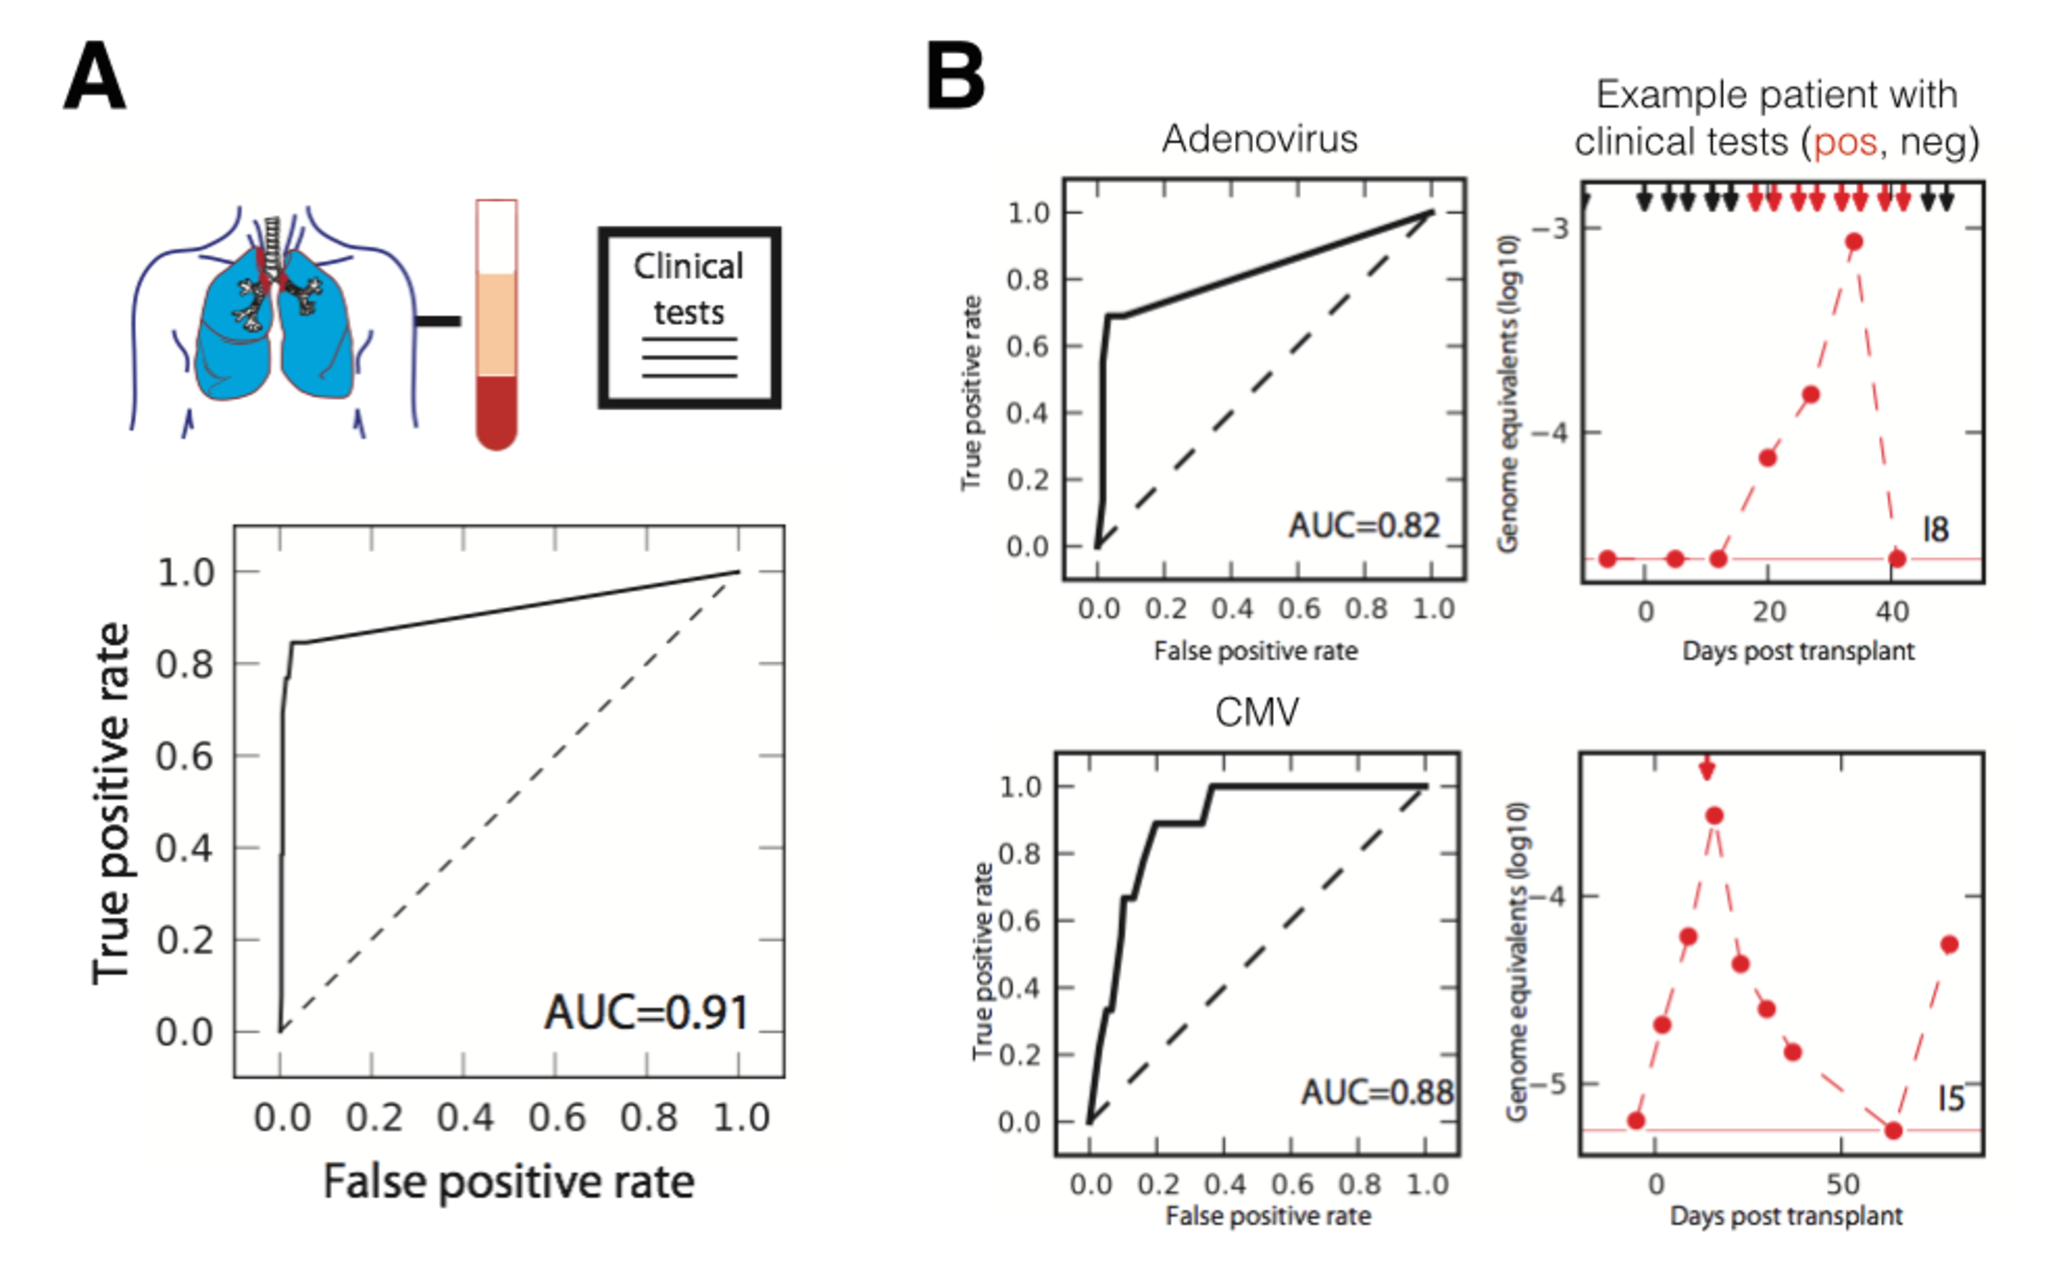
\includegraphics[width=150mm,scale=0.5]{Figures/Fig9}
\caption{Clinical correlations on viruses.}
\label{fig:Fig9}
\end{figure*}

As a result, frequent infection monitoring was performed on each transplant cohort. For the lung cohort alone, we collected over 35000 clinical measurements of specific infections performed on 14 specimen types. The majority of these measurements were specific qPCR tests for CMV, a well-known risk factor in lung transplantation, and culture applied to bronchoalveolar lavage fluid, which is used to test for deep lung bacterial infections. We evaluated whether molecular counting of infection-derived genomes in cell-free DNA correlates with clinical test for infection. 

Because there were a large number of clinical tests performed on CMV, it was a very good starting points for evaluating clinical utility of the cell-free measurements. We counted reads that map to the CMV genome for each lung transplant sample. We did this by first processing the BLAST data with an algorithm (GRAMMy) that computes relative abundance of each genome in sample based upon read mapping as well as genome size \cite{Xia:2011it}. From this data, we compute a coverage ratio for each infection relative to human, which corrects for genome size as well as sampling depth. We found that this coverage ratio correlated well with clinical tests for infection, resulting in an AUC of $0.91$ for CMV in the lung cohort (Figure ~\ref{fig:Fig9}). 

\begin{figure*}
\center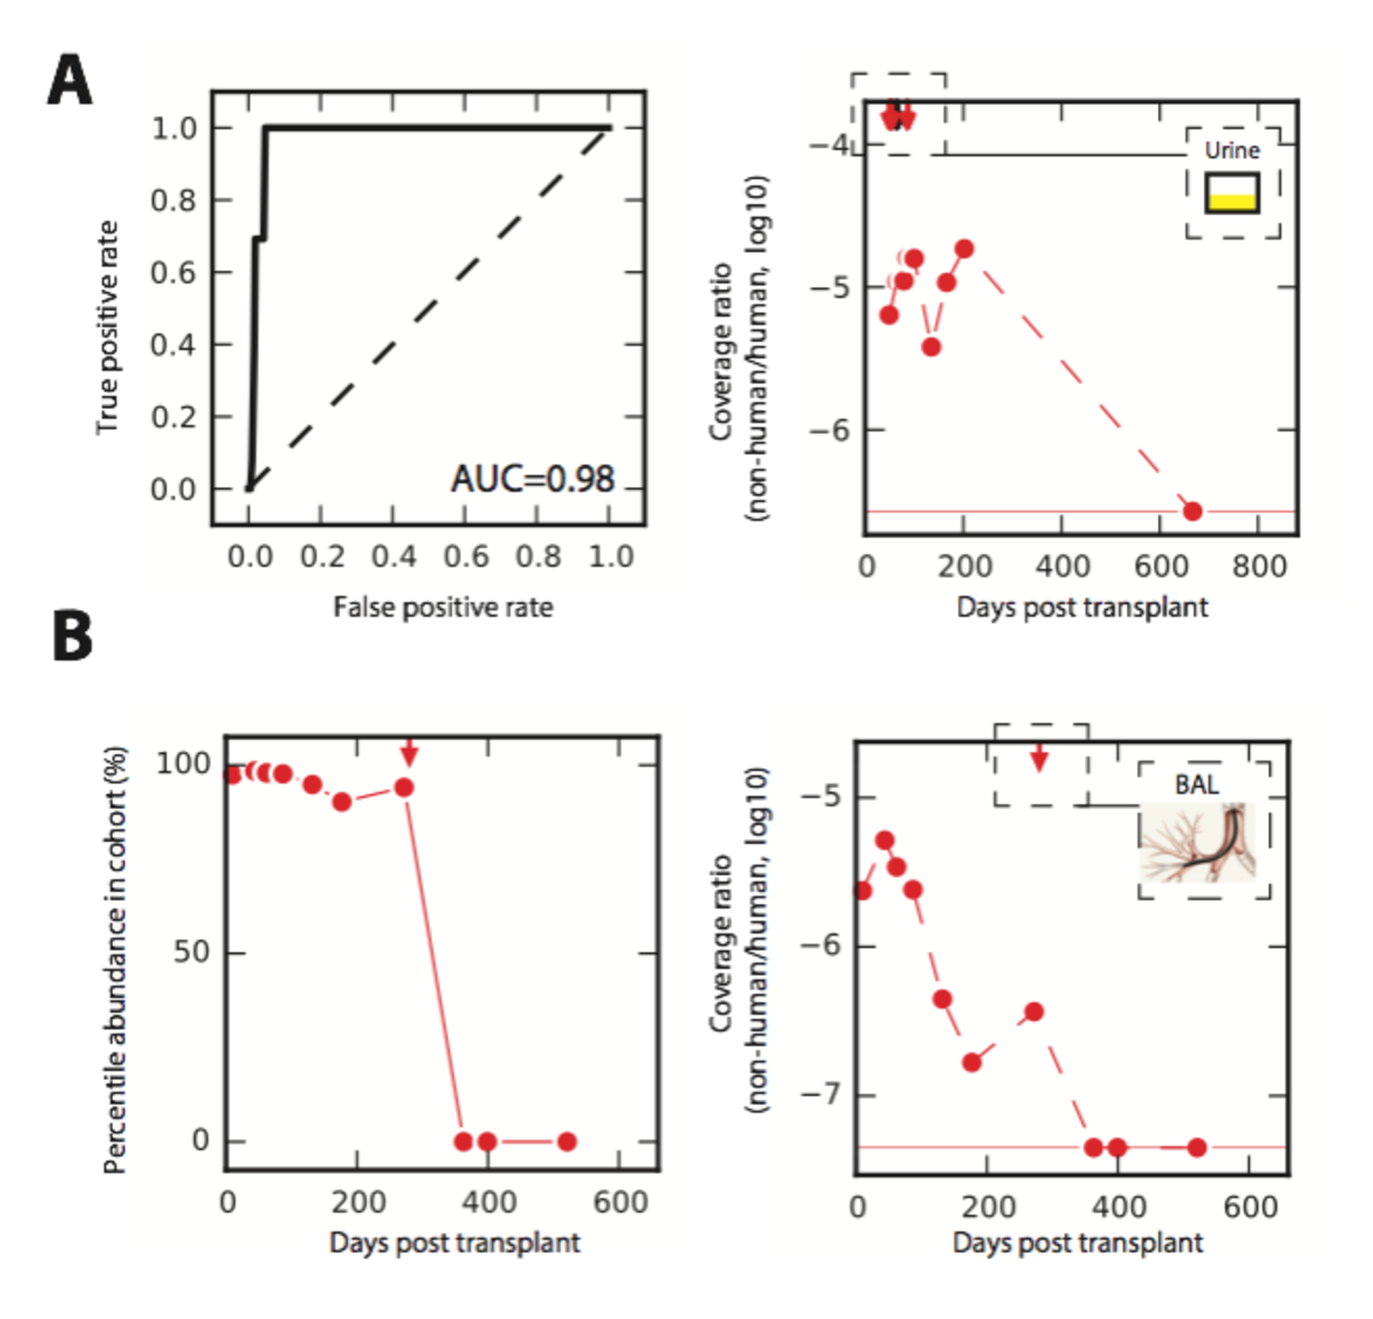
\includegraphics[width=150mm,scale=0.5]{Figures/Fig9_1}
\caption{Clinical correlations on bacteria and fungi.}
\label{fig:Fig9_1}
\end{figure*}

We then performed a similar analysis on tests collected for the pediatric bone marrow cohort. Like lung, clinical testing for CMV was common. Because of the elevated risk in the pediatric cases, this cohort also included regular screens for additional viruses, including Adenovirus (a community-acquired respiratory infection that can cause graft loss in transplant recipients and poses a particularly high risk for paediatric patients). We saw a correlation between infection-derived cfDNA and positive clinical tests in timeseries data, with elevation in signal observed when positive clinical test results were recorded (Figure ~\ref{fig:Fig9}). Cohort-level with ROC curves had AUC values of $0.82$ and $0.88$ for Adenovirus and CMV, respectively. 

The performance on viruses is encouraging, because the cell-free DNA samples used in this study were enriched: the majority of the reads were human, leaving few reads that could have been sampled from infections present in the blood. The fact that we observed correlation in the face of this limitation is remarkable. A far better signal should be achieved when human-depletion strategies are employed. 

In addition to viruses measured in serum, we also observed an agreement between cell-free DNA measurements and fungi and bacteria detected in other body fluids, including \emph{Klebsiella Pneumonia} infections detected via urine culture (ROC = 0.98) and \emph{Aspergillus Niger} infection detected in BAL  (Figure ~\ref{fig:Fig9_1}). In the case of \emph{Klebsiella}, there were 687 negative results and 13 positive results. All positive test results are in L24, and (except 1 for BAL) and are detected in urine, resulting in a consistent timeseries in our data that agrees with clinical results. Matched sample-tests data for \emph{Aspergillus Niger}, which has 481 negative results and 2 positive results in L17 (1 BAL and 1 sputum) with the single test for BAL is shown.  The percentile measurement highlights that measurements in L24 are large relative to the cohort, which is consistent with the positive clinical test results in this patient.

\begin{figure*}
\center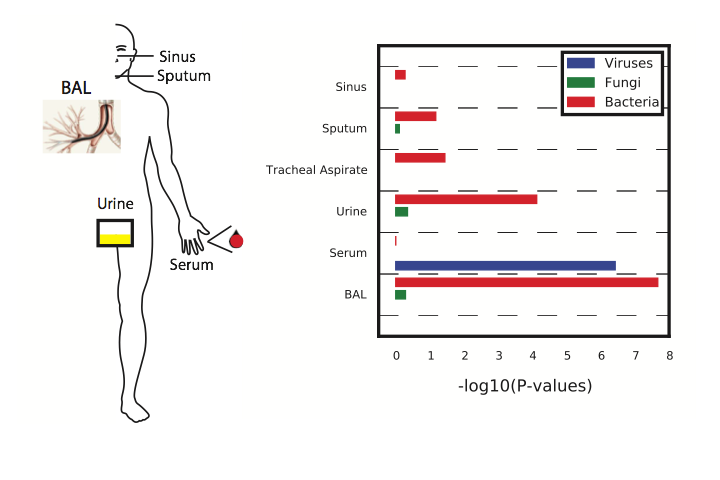
\includegraphics[width=150mm,scale=0.5]{Figures/Fig9_2}
\caption{Clinical correlations across sample types.}
\label{fig:Fig9_2}
\end{figure*}

We also evaluated the performance on classes of pathogen as well as sample type. The performance of bacterial and fungal correlations depended both on the infection type as well as the body site queried. In general, we observed better performance for body sites that have tighter coupling to blood (Figure \ref{fig:Fig9_2}). We also found that the assay performance depends on the level of the normal background signal. For example, test performance for the most commonly cultured bacteria (Pseudomonas), detected in over 80\% of the patient samples was poor (AUC 0.62) in contrast to test performance for the most commonly detected viral pathogen (CMV), detected in only 6\% of our patient samples (AUC 0.91). This highlights an important caveat in the ability of the plasma DNA sequencing for the detection of unusual abundance of commensal organisms (including Pseudomonas). Because they are part of the normal flora, many body site may contribute to the signal observed in blood and observe tissue-specific infection or dysbiosis due to pathology.

\begin{figure*}
\center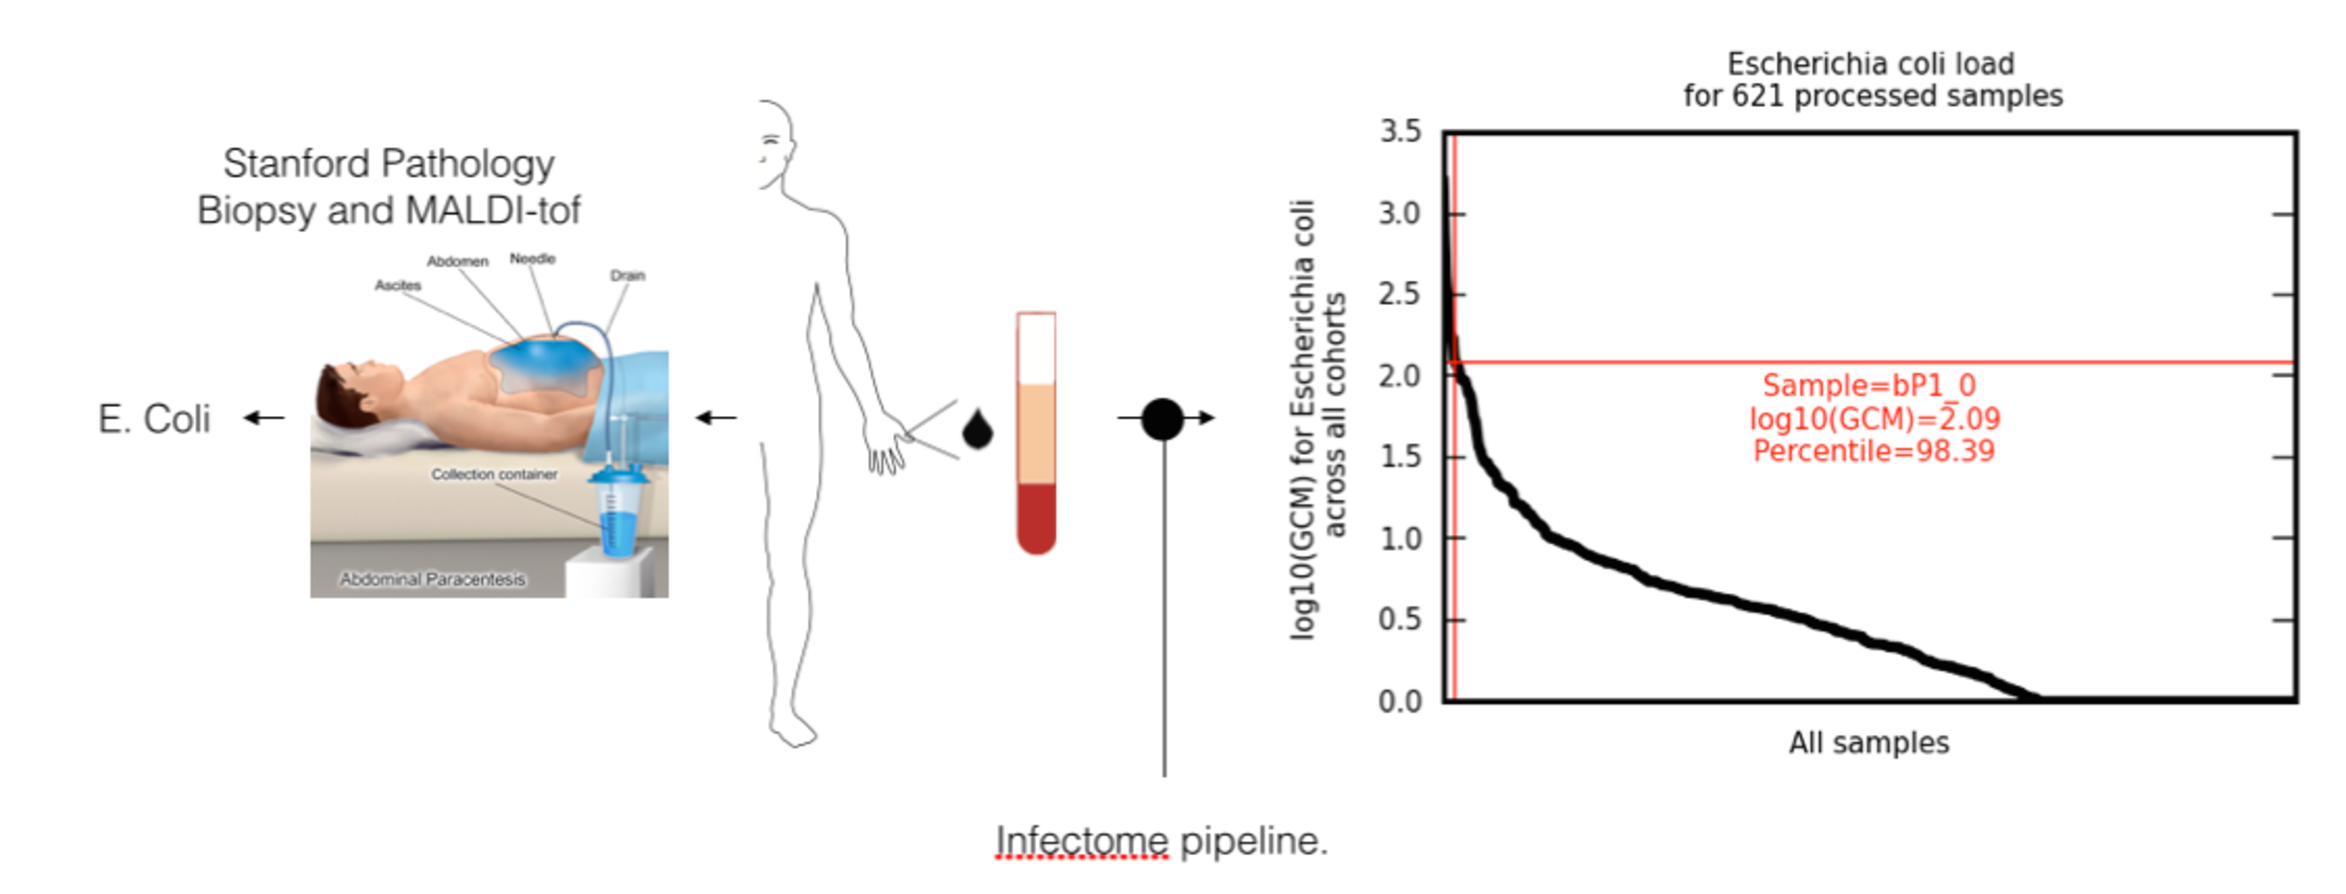
\includegraphics[width=150mm,scale=0.5]{Figures/Fig10}
\caption{Clinical correlations with deep tissue sampling}
\label{fig:Fig10}
\end{figure*}

\section{Deep tissues}

We next examined whether molecular counting of infection-derived cell-free DNA correlates with tests for deep-tissue infections. This would be appealing, because invasive biopsies are risky, particularly in patients with compromised heath. We obtained blood samples from patients with deep tissue infections, which had biopsy performed and screened using MALDI-tof. We observed favorable correlation on the cohort in a pilot test of four samples. For example, on a patient with a gastrointestinal abcess  that tested positive for \emph{E. Coli}, we measured a very high ($98\%$) percentile measurement of  \emph{E. Coli} in plasma for this patient relative to all other (> 700) samples processed (Figure ~\ref{fig:Fig10}). In turn, this provides evidence that non-viral infections in deep tissues can be detected non-invasively via molecular counting.

\section{Untested infections}

\begin{figure*}
\center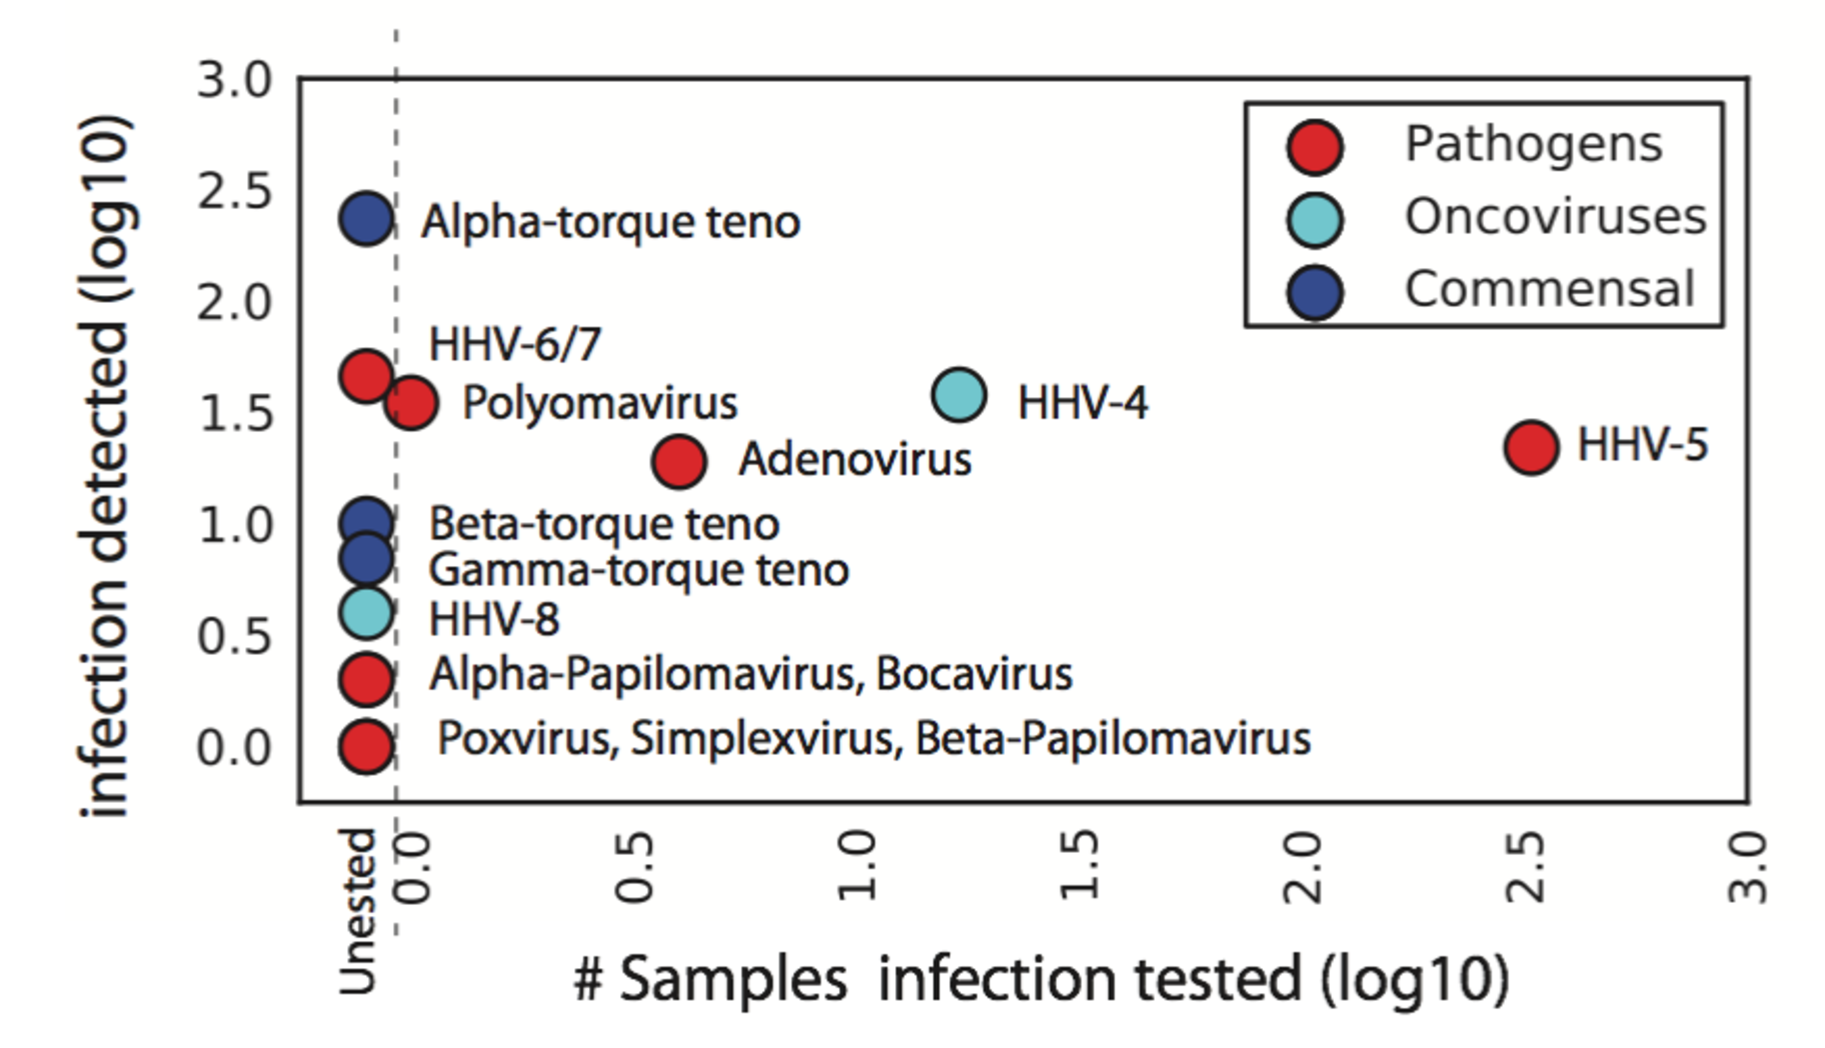
\includegraphics[width=150mm,scale=0.5]{Figures/Fig11}
\caption{Clinical correlations on viruses}
\label{fig:Fig11}
\end{figure*}

The benefit of unbiased molecular counting of infectious agents is particularly appealing, because it can indicate agents that currently fall outside the scope of clinical testing. We examined the merits of hypothesis-free screening by re-visiting our measurements relative to the recorded clinical data in the lung transplant cohort. In our data, we identified a host of viruses, ranging from well characterized pathogenic and onco-viruses to commensal torque teno viruses. The frequency of clinical testing for these viruses varied considerably, with frequent surveillance of CMV (Human Herpes Virus 5, HHV-5) relative to all other pathogens (Figure ~\ref{fig:Fig11}). 

We evaluated the incidence of infection (number of samples in which a given virus is detected via sequencing) relative to the clinical screening frequency. Although CMV was screened for most frequently (335 samples), its incidence determined by sequencing (detected in 22 samples) was similar to that of other pathogens that were not routinely screened, including adenovirus and polyomavirus (clinically tested on four occasions and one occasion, respectively). We further found that unbiased monitoring revealed numerous un-tested pathogens, including un-diagnosed cases of adenovirus, polyomavius, HHV-8, and microsporidia in patients who had similar microbial cfDNA levels compared to patients with positive clinical test results and associated symptoms. With this mind, unbiased screening is a powerful compliment to existing, hypothesis-centric clinical tests for infection.
